% Options for packages loaded elsewhere
\PassOptionsToPackage{unicode}{hyperref}
\PassOptionsToPackage{hyphens}{url}
%
\documentclass[
]{article}
\usepackage{amsmath,amssymb}
\usepackage{lmodern}
\usepackage{ifxetex,ifluatex}
\ifnum 0\ifxetex 1\fi\ifluatex 1\fi=0 % if pdftex
  \usepackage[T1]{fontenc}
  \usepackage[utf8]{inputenc}
  \usepackage{textcomp} % provide euro and other symbols
\else % if luatex or xetex
  \usepackage{unicode-math}
  \defaultfontfeatures{Scale=MatchLowercase}
  \defaultfontfeatures[\rmfamily]{Ligatures=TeX,Scale=1}
\fi
% Use upquote if available, for straight quotes in verbatim environments
\IfFileExists{upquote.sty}{\usepackage{upquote}}{}
\IfFileExists{microtype.sty}{% use microtype if available
  \usepackage[]{microtype}
  \UseMicrotypeSet[protrusion]{basicmath} % disable protrusion for tt fonts
}{}
\makeatletter
\@ifundefined{KOMAClassName}{% if non-KOMA class
  \IfFileExists{parskip.sty}{%
    \usepackage{parskip}
  }{% else
    \setlength{\parindent}{0pt}
    \setlength{\parskip}{6pt plus 2pt minus 1pt}}
}{% if KOMA class
  \KOMAoptions{parskip=half}}
\makeatother
\usepackage{xcolor}
\IfFileExists{xurl.sty}{\usepackage{xurl}}{} % add URL line breaks if available
\IfFileExists{bookmark.sty}{\usepackage{bookmark}}{\usepackage{hyperref}}
\hypersetup{
  pdftitle={lab2\_1\_fix.R},
  pdfauthor={Linne},
  hidelinks,
  pdfcreator={LaTeX via pandoc}}
\urlstyle{same} % disable monospaced font for URLs
\usepackage[margin=1in]{geometry}
\usepackage{graphicx}
\makeatletter
\def\maxwidth{\ifdim\Gin@nat@width>\linewidth\linewidth\else\Gin@nat@width\fi}
\def\maxheight{\ifdim\Gin@nat@height>\textheight\textheight\else\Gin@nat@height\fi}
\makeatother
% Scale images if necessary, so that they will not overflow the page
% margins by default, and it is still possible to overwrite the defaults
% using explicit options in \includegraphics[width, height, ...]{}
\setkeys{Gin}{width=\maxwidth,height=\maxheight,keepaspectratio}
% Set default figure placement to htbp
\makeatletter
\def\fps@figure{htbp}
\makeatother
\setlength{\emergencystretch}{3em} % prevent overfull lines
\providecommand{\tightlist}{%
  \setlength{\itemsep}{0pt}\setlength{\parskip}{0pt}}
\setcounter{secnumdepth}{-\maxdimen} % remove section numbering
\ifluatex
  \usepackage{selnolig}  % disable illegal ligatures
\fi

\title{lab2\_1\_fix.R}
\author{Linne}
\date{2022-12-05}

\begin{document}
\maketitle

\begin{verbatim}
## [1] "Test error"
\end{verbatim}

\begin{verbatim}
## [1] 722.4294
\end{verbatim}

\begin{verbatim}
## [1] "Train error"
\end{verbatim}

\begin{verbatim}
## [1] 0.005709117
\end{verbatim}

\includegraphics{lab2_1_fix_files/figure-latex/unnamed-chunk-2-1.png}
\includegraphics{lab2_1_fix_files/figure-latex/unnamed-chunk-3-1.pdf}
\includegraphics{lab2_1_fix_files/figure-latex/unnamed-chunk-4-1.pdf}
\includegraphics{lab2_1_fix_files/figure-latex/unnamed-chunk-4-2.pdf}

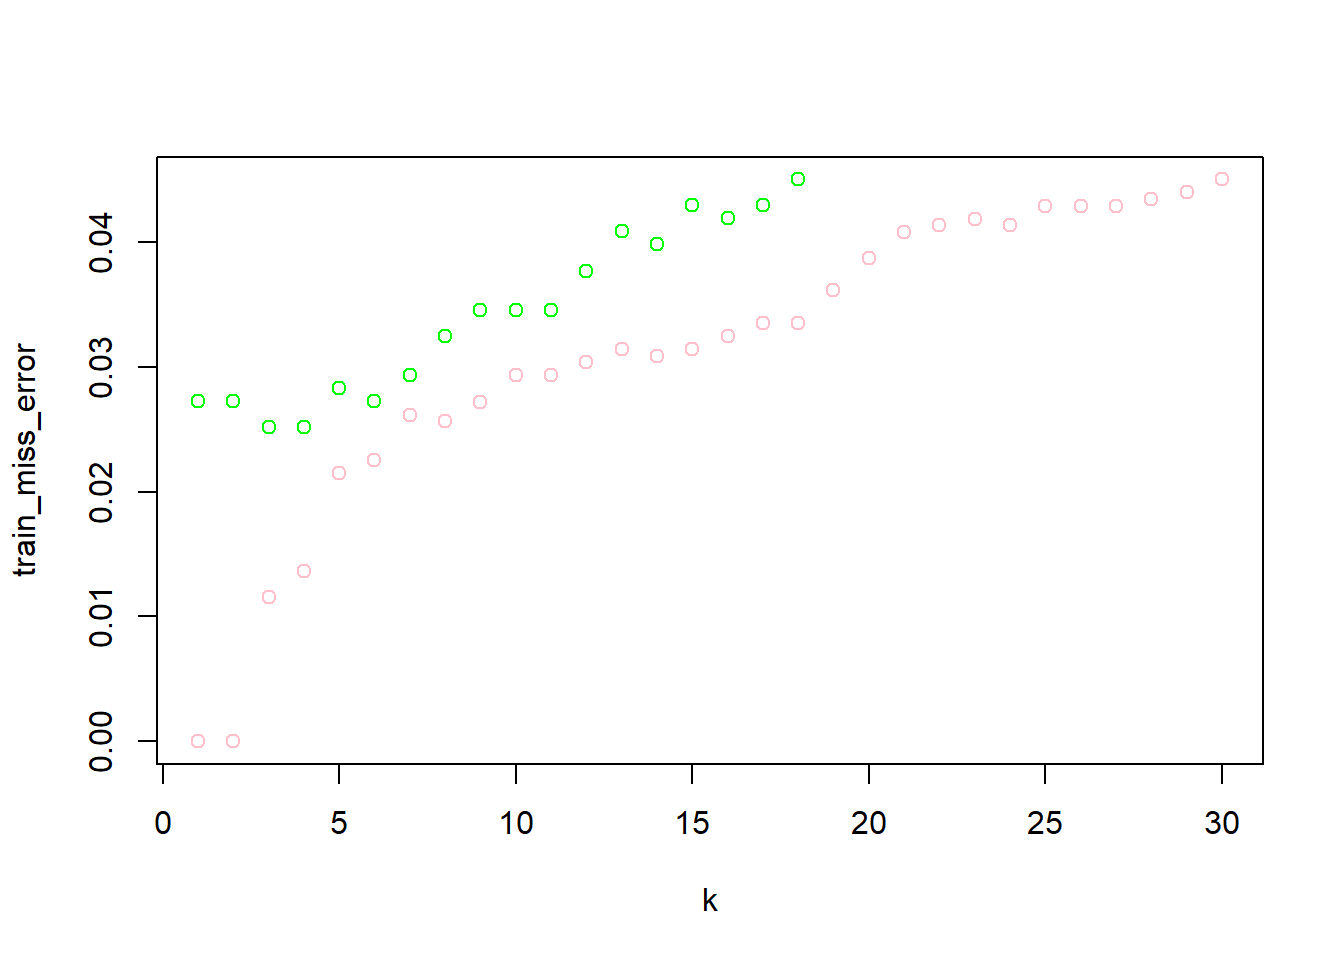
\includegraphics{lab2_1_fix_files/figure-latex/unnamed-chunk-6-1.pdf}
\includegraphics{lab2_1_fix_files/figure-latex/unnamed-chunk-6-2.pdf}
\includegraphics{lab2_1_fix_files/figure-latex/unnamed-chunk-6-3.pdf}

\begin{verbatim}
## [1] "1) Training and validation"
\end{verbatim}

\begin{verbatim}
## [1] 0.1048441
\end{verbatim}

\begin{verbatim}
## [1] 0.1092679
\end{verbatim}

\begin{verbatim}
## [1] "2) Training and validation"
\end{verbatim}

\begin{verbatim}
## [1] 0.1048441
\end{verbatim}

\begin{verbatim}
## [1] 0.1092679
\end{verbatim}

\begin{verbatim}
## [1] "3) Training and validation"
\end{verbatim}

\begin{verbatim}
## [1] 0.09400575
\end{verbatim}

\begin{verbatim}
## [1] 0.1119221
\end{verbatim}

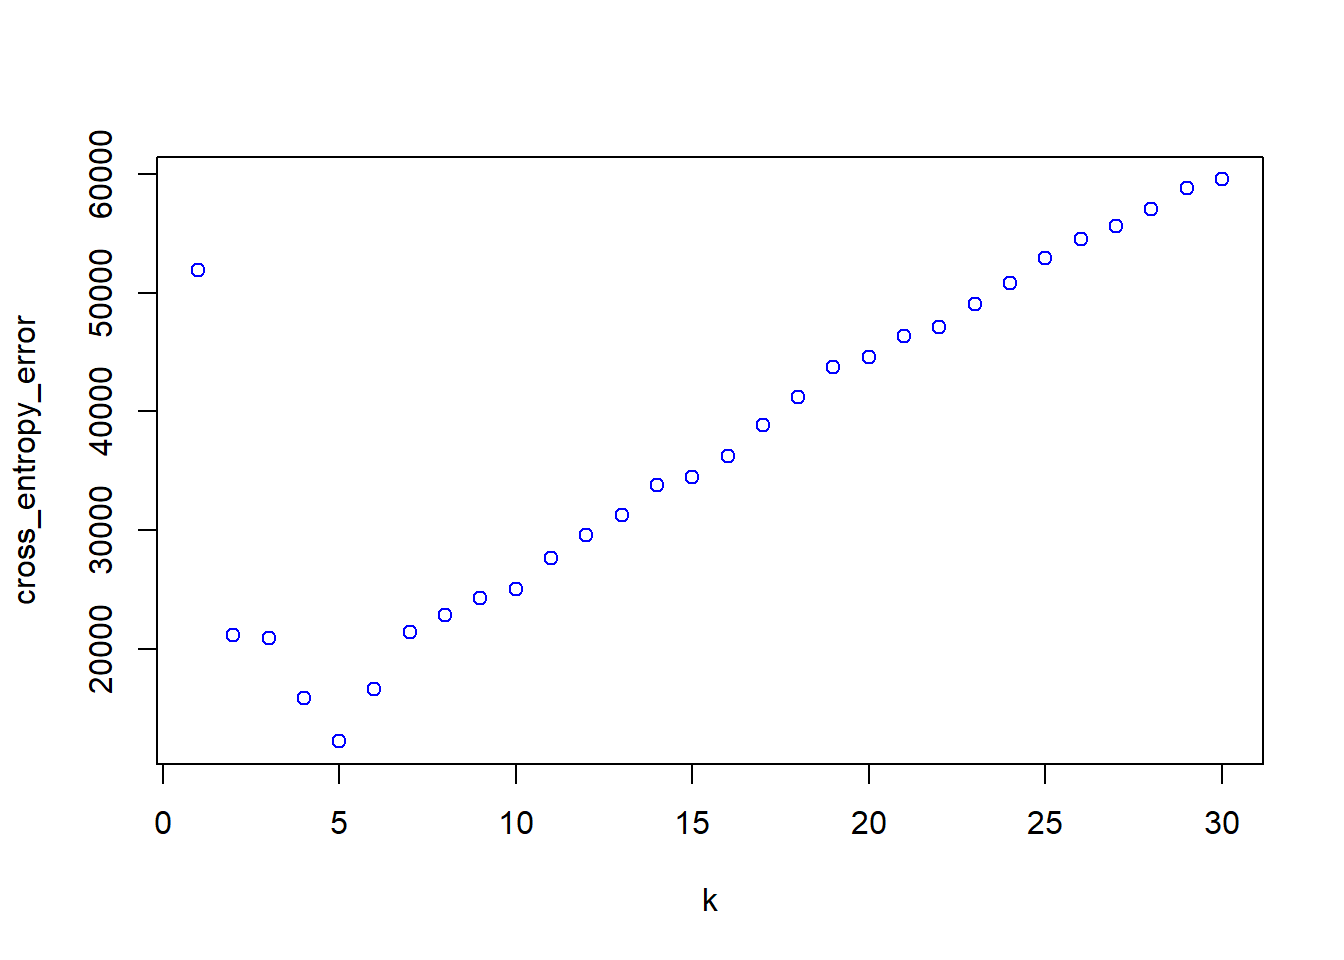
\includegraphics{lab2_1_fix_files/figure-latex/unnamed-chunk-8-1.pdf}

\begin{verbatim}
## [1] 21
\end{verbatim}

\includegraphics{lab2_1_fix_files/figure-latex/unnamed-chunk-8-2.pdf}

\includegraphics{lab2_1_fix_files/figure-latex/unnamed-chunk-11-1.pdf}
\includegraphics{lab2_1_fix_files/figure-latex/unnamed-chunk-11-2.pdf}

\begin{verbatim}
## [1] 34
\end{verbatim}

\begin{verbatim}
## [1] 0.2501699 0.1693597
\end{verbatim}

\begin{verbatim}
##      medFamInc      medIncome    PctKids2Par     pctWInvInc PctPopUnderPov 
##     -0.1833080     -0.1819830     -0.1755423     -0.1748683      0.1737978
\end{verbatim}

\includegraphics{lab2_1_fix_files/figure-latex/unnamed-chunk-13-1.pdf}

\begin{verbatim}
## [1] "Train error"
\end{verbatim}

\begin{verbatim}
## [1] 0.2591772
\end{verbatim}

\begin{verbatim}
## [1] "Test error"
\end{verbatim}

\begin{verbatim}
## [1] 0.4000579
\end{verbatim}

\begin{verbatim}
## [1] "calculated optimal train"
\end{verbatim}

\begin{verbatim}
## [1] 0.2592247
\end{verbatim}

\begin{verbatim}
## [1] "Lm train error"
\end{verbatim}

\begin{verbatim}
## [1] 0.2591772
\end{verbatim}

\begin{verbatim}
## [1] "calculated optimal test"
\end{verbatim}

\begin{verbatim}
## [1] 0.3997238
\end{verbatim}

\begin{verbatim}
## [1] "Lm test error"
\end{verbatim}

\begin{verbatim}
## [1] 0.4000579
\end{verbatim}

\begin{verbatim}
## [1] "Early stopping index and MSE"
\end{verbatim}

\begin{verbatim}
## [1] 2183
\end{verbatim}

\begin{verbatim}
## [1] 0.3769468
\end{verbatim}

\includegraphics{lab2_1_fix_files/figure-latex/unnamed-chunk-15-1.pdf}

\end{document}
